\documentclass{beamer}
\usepackage{multimedia}
\usepackage{hyperref}
\usepackage{longtable,booktabs}
\usepackage{subcaption,siunitx}
\usepackage{scrextend}
\usepackage{tablefootnote}

%\usepackage{graphicx}
%\usepackage{epstopdf}

\usepackage[backend=bibtex,style=verbose]{biblatex}
\addbibresource{mybibfile.bib}

% Define headline format
\setbeamertemplate{headline}
{ %scshape
   \leavevmode%
   \hbox{%
   \begin{beamercolorbox}[wd=.5\paperwidth,ht=2.25ex,dp=1ex,left]{section in head/foot}%
     \usebeamerfont{section in head/foot}\hspace*{3ex}\MakeUppercase\insertsectionhead
   \end{beamercolorbox}%
   \begin{beamercolorbox}[wd=.5\paperwidth,ht=3.25ex,dp=1ex,right]{subsection in head/foot}%
     \usebeamerfont{subsection in head/foot}\MakeUppercase\insertsubsectionhead\hspace*{3ex}
   \end{beamercolorbox}}%
   \vskip0pt%
}

\beamertemplatenavigationsymbolsempty

% Reduce the margin-top of the title of every slide
\setbeamertemplate{frametitle}{
    \vspace{0cm}
    \insertframetitle
}

% Change footnote default fontsize
\setbeamerfont{footnote}{size=\tiny}

% Change caption default fontsize
\setbeamerfont{caption}{size=\scriptsize}




\begin{document}


\title{Beating human performance at recognizing speech commands in temporal domain}
\author[UV]{Iván Vallés-Pérez, Fernando Mateo, Joan Vila-Francés, Antonio J. Serrano-López, Emilio Soria-Olivas}
\institute[UV]{Escola Tècnica Superior d\textsc{\char13}Enginyeria, University of Valencia, Avenida de la Universitat s/n 46100 Burjassot, Valencia, Spain}

\date{July 20th, 2020}

% --------------------------------------------- NEW SLIDE ------------------------------
\frame{\titlepage}

\section{Introduction}

\frame{\frametitle{The field of voice-activated virtual assistants is booming}
    \begin{itemize}
    \item Several big companies like Amazon, Google, Baidu and Apple have already developed their version of virtual assistant
    \item In particular, Deep Learning (DL) models have revolutionized the field of automatic speech recognition \footfullcite{Nassif2019}, as language features are highly hierarchical.
    \item There are multiple open research lines.
    \begin{itemize}
        \item Increasing the accuracy and relevance of the responses \footfullcite{milabot2017}
        \item Reducing the answer delay \footfullcite{Han2017}
        \item Increasing their variability of the responses \footfullcite{Li2017}
        \item ...
    \end{itemize}
    \end{itemize}
}

% --------------------------------------------- NEW SLIDE ------------------------------
\frame{\frametitle{This work focuses on increasing the accuracy of the voice commands recognition}
\begin{itemize}
    \item The \textbf{objective} of this project is to achieve the best possible accuracy on the recognition of speech commands under a limited vocabulary setting
    \item For that, we propose using Deep Learning techniques – more specifically: \textbf{convolutional neural networks}
    \item No complex pre-processing techniques (such as \textit{FFT} and spectrograms) are intended to be applied to the audio clips: we are going to stay in the \textbf{temporal domain}
    \item To quantify the performance of the solution, we will not only measure against existing \textbf{benchmarks}, but also against manually measured \textbf{human accuracy}
\end{itemize}
}

\section{Data}
% --------------------------------------------- NEW SLIDE ------------------------------
\frame{\frametitle{The Google Tensorflow speech commands data set has been used to perform this study}
    \small
    \begin{itemize}
        \item \textit{Google Tensorflow speech commands data set}\footfullcite{speechcommands} is a collection of categorized audio utterances released by Google in 2018
        \item Noisy and low-quality audio clips, recoded in uncontrolled environments
        \item More than 100,000 1s-length audio clips belonging to 35 different classes\footnote{According to version 2 of the data set. Version 1 contains around 65,000 clips and 30 different classes}
        \item Two versions of the data set are available, where V2 is an extended and cleaned version of V1. Results have been reported on both versions of the data set

    \end{itemize}

    \movie[inlinesound, samplingrate=16000, showcontrols=false]{[left]}{audio/originals/left.wav},
    \movie[inlinesound, samplingrate=16000, showcontrols=false]{[right]}{audio/originals/right.wav},
    \movie[inlinesound, samplingrate=16000, showcontrols=false]{[yes]}{audio/originals/yes.wav},
    \movie[inlinesound, samplingrate=16000, showcontrols=false]{[no]}{audio/originals/no.wav},
    \movie[inlinesound, samplingrate=16000, showcontrols=false]{[down]}{audio/originals/down.wav},
    \movie[inlinesound, samplingrate=16000, showcontrols=false]{[up]}{audio/originals/up.wav},
    \movie[inlinesound, samplingrate=16000, showcontrols=false]{[go]}{audio/originals/go.wav},
    \movie[inlinesound, samplingrate=16000, showcontrols=false]{[stop]}{audio/originals/stop.wav},
    \movie[inlinesound, samplingrate=16000, showcontrols=false]{[on]}{audio/originals/on.wav},
    \movie[inlinesound, samplingrate=16000, showcontrols=false]{[off]}{audio/originals/off.wav},
    \movie[inlinesound, samplingrate=16000, showcontrols=false]{[zero]}{audio/originals/zero.wav},
    \movie[inlinesound, samplingrate=16000, showcontrols=false]{[one]}{audio/originals/one.wav},
    \movie[inlinesound, samplingrate=16000, showcontrols=false]{[two]}{audio/originals/two.wav},
    \movie[inlinesound, samplingrate=16000, showcontrols=false]{[three]}{audio/originals/three.wav},
    \movie[inlinesound, samplingrate=16000, showcontrols=false]{[four]}{audio/originals/four.wav},
    \movie[inlinesound, samplingrate=16000, showcontrols=false]{[five]}{audio/originals/five.wav},
    \movie[inlinesound, samplingrate=16000, showcontrols=false]{[six]}{audio/originals/six.wav},
    \movie[inlinesound, samplingrate=16000, showcontrols=false]{[seven]}{audio/originals/seven.wav},
    \movie[inlinesound, samplingrate=16000, showcontrols=false]{[eight]}{audio/originals/eight.wav},
    \movie[inlinesound, samplingrate=16000, showcontrols=false]{[nine]}{audio/originals/nine.wav},
    \movie[inlinesound, samplingrate=16000, showcontrols=false]{[dog]}{audio/originals/dog.wav},
    \movie[inlinesound, samplingrate=16000, showcontrols=false]{[cat]}{audio/originals/cat.wav},
    \movie[inlinesound, samplingrate=16000, showcontrols=false]{[wow]}{audio/originals/wow.wav},
    \movie[inlinesound, samplingrate=16000, showcontrols=false]{[house]}{audio/originals/house.wav},
    \movie[inlinesound, samplingrate=16000, showcontrols=false]{[bird]}{audio/originals/bird.wav},
    \movie[inlinesound, samplingrate=16000, showcontrols=false]{[happy]}{audio/originals/happy.wav},
    \movie[inlinesound, samplingrate=16000, showcontrols=false]{[sheila]}{audio/originals/sheila.wav},
    \movie[inlinesound, samplingrate=16000, showcontrols=false]{[marvin]}{audio/originals/marvin.wav},
    \movie[inlinesound, samplingrate=16000, showcontrols=false]{[bed]}{audio/originals/bed.wav},
    \movie[inlinesound, samplingrate=16000, showcontrols=false]{[tree]}{audio/originals/tree.wav},
    \movie[inlinesound, samplingrate=16000, showcontrols=false]{[visual]}{audio/originals/visual.wav},
    \movie[inlinesound, samplingrate=16000, showcontrols=false]{[follow]}{audio/originals/follow.wav},
    \movie[inlinesound, samplingrate=16000, showcontrols=false]{[learn]}{audio/originals/learn.wav},
    \movie[inlinesound, samplingrate=16000, showcontrols=false]{[forward]}{audio/originals/forward.wav},
    \movie[inlinesound, samplingrate=16000, showcontrols=false]{[backward]}{audio/originals/backward.wav}
}

% --------------------------------------------- NEW SLIDE ------------------------------
\frame{\frametitle{Classifying speech commands at temporal domain is not straightforward}
\begin{columns}
    \begin{column}{0.5\textwidth}
        \begin{figure}[h!]
            \centering
            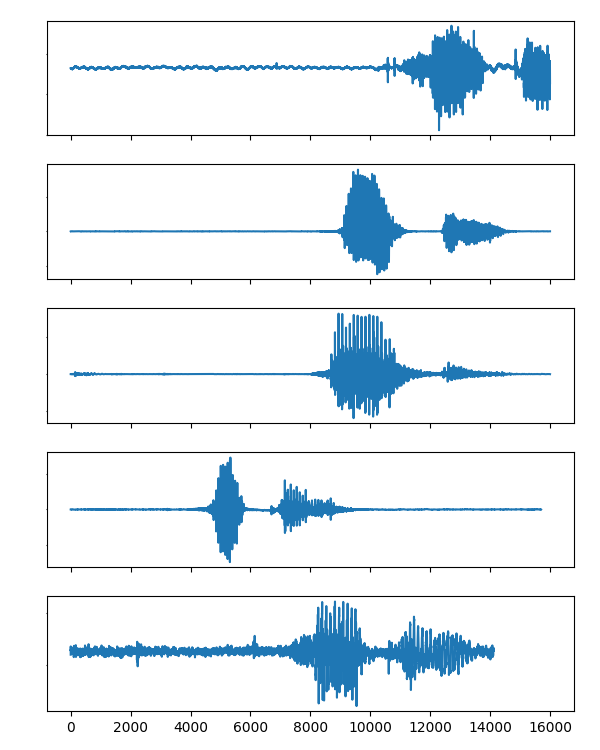
\includegraphics[width=.95\linewidth]{img/happy}
            \caption{Happy:
            \movie[inlinesound, samplingrate=16000, showcontrols=false]{[1]}{audio/comp/happy_0.wav},
                \movie[inlinesound, samplingrate=16000, showcontrols=false]{[2]}{audio/comp/happy_1.wav},
                \movie[inlinesound, samplingrate=16000, showcontrols=false]{[3]}{audio/comp/happy_2.wav},
                \movie[inlinesound, samplingrate=16000, showcontrols=false]{[4]}{audio/comp/happy_3.wav},
                \movie[inlinesound, samplingrate=16000, showcontrols=false]{[5]}{audio/comp/happy_4.wav}}
        \end{figure}
    \end{column}
    \begin{column}{0.5\textwidth}
        \begin{figure}[h!]
            \centering
            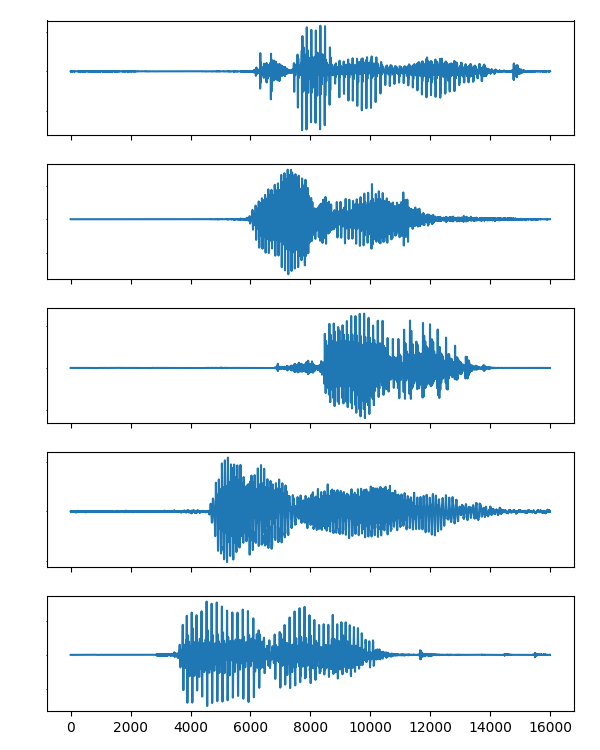
\includegraphics[width=.95\linewidth]{img/forward}
            \caption{Forward:
            \movie[inlinesound, samplingrate=16000, showcontrols=false]{[1]}{audio/comp/forward_0.wav},
            \movie[inlinesound, samplingrate=16000, showcontrols=false]{[2]}{audio/comp/forward_1.wav},
            \movie[inlinesound, samplingrate=16000, showcontrols=false]{[3]}{audio/comp/forward_2.wav},
            \movie[inlinesound, samplingrate=16000, showcontrols=false]{[4]}{audio/comp/forward_3.wav},
            \movie[inlinesound, samplingrate=16000, showcontrols=false]{[5]}{audio/comp/forward_4.wav}}
        \end{figure}
    \end{column}
\end{columns}
}

% --------------------------------------------- NEW SLIDE ------------------------------
\frame{\frametitle{Four different tasks have been defined with the available data for benchmarking purposes}

    \begin{itemize}
        \item We defined a set of ``tasks'' by pre-selecting a subset of the classes and assigning the others to a synthetic ``unknown class''.
        \item This groups have been established to be able to compare with the existing SOTA benchmarks \footfullcite{Andrade2018} \footfullcite{McMahan2018} \footfullcite{Warden2018} \footfullcite{Zhang2017}.
        \begin{enumerate}[a.]
            \item \textit{35-words-recognition}
            \item \textit{20-commands-recognition} + \textit{unknown}
            \item \textit{10-commands-recognition} + \textit{unknown}
            \item \textit{left-right} + \textit{unknown}
        \end{enumerate}
    \end{itemize}

}

% --------------------------------------------- NEW SLIDE ------------------------------
\frame{\frametitle{Four different tasks have been defined with the available data for benchmarking purposes}
\begin{figure}[h!]
    \centering
    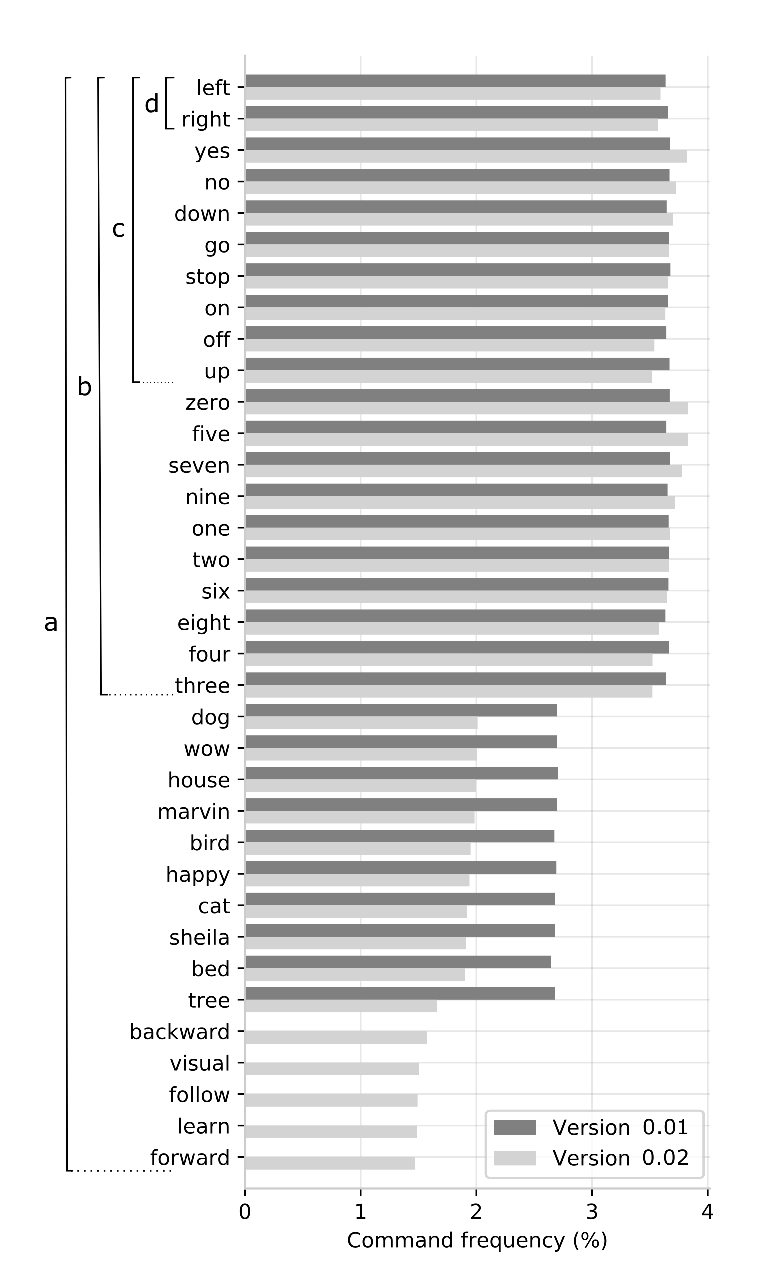
\includegraphics[height=0.5\linewidth]{img/freqdist_data}
	\caption{Command frequency distribution for both versions of the data set. As it can be noticed, the V2 is a refined and extended version of V1. In the left, the four different tasks that have been benchmarked in this work: (a) referred as \textit{35-words-recognition} and comprising in both cases all the words for classification, (b) referred as \textit{20-commands-recognition}  (c) referred as \textit{10-commands-recognition} (d) referred as \textit{left-right} recognition.}
    \label{fig:freqdistdata}
\end{figure}
}

% --------------------------------------------- NEW SLIDE ------------------------------
\frame{\frametitle{As we group the unrecognized words under the ``unknown'' category, the class imbalance grows}
\small
\begin{itemize}
    \item The \textbf{cost of a false positive} in a speech recognition agent is \textbf{higher} than that of a false negative
    \item The precision should be optimized at the expense of a worse recall
    \item Thus, having a positive imbalance towards the ``unknown'' class does not represent a very big inconvenience
\end{itemize}
\footnotesize
\begin{table}[h!]
	\centering
	\caption{Percentage of words represented by the ``unknown'' category in each one of the proposed speech recognition tasks. }
	\label{tab:unknowns}
	\begin{tabular}{lcccc}
		\hline
		Data set version & \textit{35-words} & \textit{20-commands} & \textit{10-commands} & \textit{left-right}  \\
		\hline
		V1 	& 0.00$\%$  &  26.84$\%$  &	  63.41$\%$  &	92.71$\%$ \\
		V2 	& 0.00$\%$  &	26.81$\%$  &  63.58$\%$  &	92.84$\%$ \\
		\bottomrule
	\end{tabular}
\end{table}

}

% --------------------------------------------- NEW SLIDE ------------------------------
\frame{\frametitle{Several data augmentation techniques have been used to enhance generalization}
    \small
    The \movie[inlinesound, samplingrate=16000, showcontrols=false]{[original]}{audio/distorted/original.wav} data set has been augmented through the random application of 5 different distortions \footfullcite{Proakis2007}:
    \begin{itemize}
        \item \textbf{Resampling}: expanding and contracting the audio clip + center-cropping. Examples:
        \movie[inlinesound, samplingrate=16000, showcontrols=false]{[1]}{audio/distorted/resample_0.wav}
        \movie[inlinesound, samplingrate=16000, showcontrols=false]{[2]}{audio/distorted/resample_1.wav}
        \movie[inlinesound, samplingrate=16000, showcontrols=false]{[3]}{audio/distorted/resample_4.wav}
        \item \textbf{Pitch shift}: frequency increase/decrease to produce more acute/severe voices. Examples:
        \movie[inlinesound, samplingrate=16000, showcontrols=false]{[1]}{audio/distorted/pitch_shift_0.wav}
        \movie[inlinesound, samplingrate=16000, showcontrols=false]{[2]}{audio/distorted/pitch_shift_1.wav}
        \movie[inlinesound, samplingrate=16000, showcontrols=false]{[3]}{audio/distorted/pitch_shift_3.wav}
        \item \textbf{Saturation}: amplitude increase until saturation. Examples:
        \movie[inlinesound, samplingrate=16000, showcontrols=false]{[1]}{audio/distorted/saturate_3.wav}
        \movie[inlinesound, samplingrate=16000, showcontrols=false]{[2]}{audio/distorted/saturate_1.wav}
        \movie[inlinesound, samplingrate=16000, showcontrols=false]{[3]}{audio/distorted/saturate_2.wav}
        \item \textbf{Time offset}: left or right zero padding. Examples:
        \movie[inlinesound, samplingrate=16000, showcontrols=false]{[1]}{audio/distorted/time_offset_3.wav}
        \movie[inlinesound, samplingrate=16000, showcontrols=false]{[2]}{audio/distorted/time_offset_1.wav}
        \movie[inlinesound, samplingrate=16000, showcontrols=false]{[3]}{audio/distorted/time_offset_2.wav}
        \item \textbf{Noise addition}: sum of white noise on the temporal sequence. Examples:
        \movie[inlinesound, samplingrate=16000, showcontrols=false]{[1]}{audio/distorted/noise_3.wav}
        \movie[inlinesound, samplingrate=16000, showcontrols=false]{[2]}{audio/distorted/noise_1.wav}
        \movie[inlinesound, samplingrate=16000, showcontrols=false]{[3]}{audio/distorted/noise_4.wav}
    \end{itemize}
    All the distortions are applied together with random intensities only over the training data, producing 5 new transformations of the original recordings
    \movie[inlinesound, samplingrate=16000, showcontrols=false]{[1]}{audio/distorted/mix_0.wav}
    \movie[inlinesound, samplingrate=16000, showcontrols=false]{[2]}{audio/distorted/mix_1.wav}
    \movie[inlinesound, samplingrate=16000, showcontrols=false]{[3]}{audio/distorted/mix_2.wav}
    \movie[inlinesound, samplingrate=16000, showcontrols=false]{[4]}{audio/distorted/mix_3.wav}
    \movie[inlinesound, samplingrate=16000, showcontrols=false]{[5]}{audio/distorted/mix_4.wav}
}

\section{Methods}
% --------------------------------------------- NEW SLIDE ------------------------------
\frame{\frametitle{A new CNN architecture based on the Xception network has been designed}
\begin{itemize}
    \item Xception\footfullcite{FChollet2017} is a CNN-based deep learning architecture published by François Chollet (Google) in 2017 which recently achieved SOTA results in multiple computer vision tasks
    \item It uses \textit{depthwise separable convolutions} and \textit{residual connections}. Both together lead to a very efficient yet deep CNN.
    \item This algorithm is designed to work with images (2-D data). We have adapted it to work with sequences (1-D data): \textbf{Xception-1d}
\end{itemize}
}

% --------------------------------------------- NEW SLIDE ------------------------------
\frame{\frametitle{The \textit{depthwise separable convolution} operation is more efficient than the common convolution (1/2)}
\small
\begin{columns}
    \begin{column}{0.5\textwidth}
        \begin{figure}[h!]
            \centering
            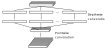
\includegraphics[width=1\linewidth]{img/dws_conv}
        \end{figure}
    \end{column}
    \begin{column}{0.5\textwidth}
        \footnotesize
        \textit{Equation \ref{eq:reg_conv}: regular convolution}
        \begin{equation}
		\mathbf{G}_{x} = \sum_{s, m} \mathbf{K}_{s, m} \cdot \mathbf{F}_{x+s-\frac{S-1}{2}, m}
            \label{eq:reg_conv}
        \end{equation}
        \textit{Equation \ref{eq:dw_conv}: depthwise convolution}
        \begin{equation}
			\hat{\mathbf{G}}_{x, m} = \sum_{s} \mathbf{K}_{s, m} \cdot \mathbf{F}_{x+s-\frac{S-1}{2}, m} 
            \label{eq:dw_conv}
        \end{equation}




    \end{column}

\end{columns}
\vspace{0.3cm}
The \textit{depthwise separable convolution} consists of two sequential steps
\begin{itemize}
    \item \textit{Depthwise convolution}\footfullcite{Yunhui2019}: single filter per channel. Modifies only spatial/temporal dimension(s). Number of channels remains intact. See equation \ref{eq:dw_conv}
    \item \textit{Pointwise convolution}\footfullcite{Gao2018}: size-1 convolutions. Modifies only the channels dimension. Spatial/temporal dimension(s) remain intact. See equation \ref{eq:reg_conv}
\end{itemize}
}

% --------------------------------------------- NEW SLIDE ------------------------------
\frame{\frametitle{The \textit{depthwise separable convolution} operation is more efficient than the common convolution (2/2)}

\begin{itemize}
    \item The \textit{depthwise separable convolution} receives its name because it \textbf{separates} the channel-wise and spatial/temporal-wise computations.
    \item The number of operations required by the depthwise-separable convolution is $\frac{1}{N} \cdot \frac{1}{S}$ \textbf{times} the number of operations required by a regular convolution \footfullcite{Howard2017} (where $N$ is the number of output channels and $S$ is the filter size), which represents a meaningful performance improvement for big networks.
    \item E.g. if we applied a size-5 convolution to generate a signal with 2 channels (e.g. a stereo audio signal), a regular convolution would need $5 * 2 = 10$ times more computation than a \textit{depthwise separable convolution}.
\end{itemize}
}
% --------------------------------------------- NEW SLIDE ------------------------------

\frame{\frametitle{37 layers have been used to define the Xception-1d architecture, with a total of 23 million parameters}
    \begin{figure}[h!]
        \centering
        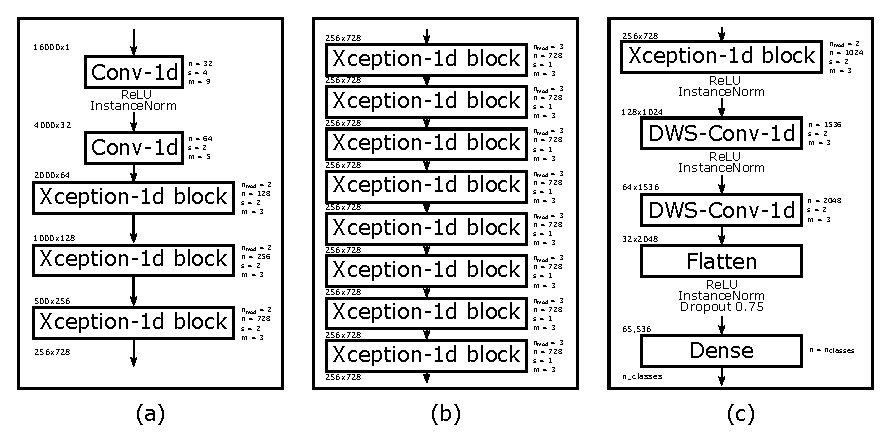
\includegraphics[width=1\linewidth]{img/arch}
        \caption{Diagram summarizing the architecture of \textit{Xception-1d}. It's composed of three main modules: (a) the entry module, responsible for adapting the raw wave into a condensed representation, (b) the middle module responsible for learning the representation for extracting useful features from the raw data, (c) the classification module, responsible for mapping the learned representation into each output class}
    \end{figure}

}

% --------------------------------------------- NEW SLIDE ------------------------------
\frame{\frametitle{The building block of the architecture is composed of two conv layers, a skip connection and a pooling layer}
    \begin{columns}
        \begin{column}{0.5\textwidth}
            \begin{itemize}
                \item Each Xception-1d block contains two chained depth-wise separable convolutions with a residual connection, followed by an average pooling layer
                \item Instance Normalization has been used as a way of reducing the covariance shift, and hence enhance generalization
                \item The skip connections of every block allows training deeper networks
            \end{itemize}
        \end{column}
        \begin{column}{0.5\textwidth}
        \begin{figure}[h!]
            \centering
            
\includegraphics[width=1\linewidth]{img/xception_module}
        \end{figure}
        \end{column}

    \end{columns}

}

% --------------------------------------------- NEW SLIDE ------------------------------
\section{Experimental design}
\frame{\frametitle{The data has been divided in train/dev/test to enable model experimentation}
\begin{itemize}
    \item The \textbf{cross-validation split} has been provided by the authors of the data set (holding about 11,000 samples for development and other about 11,000 for test purposes)
    \item The models have been trained for \textbf{50 epochs} in each case with early-stopping and the parameters have been manually tuned
    \item Five different models have been trained for each task in order to explore and report the effect of different \textbf{random initializations} of the weights of the network
    \item With the aim of providing a baseline, \textbf{human performance} has been measured by \textbf{4 human subjects}, who manually labeled \textbf{1000 commands}
    \item The source code of this study is publicly available on \textbf{GitHub}:  https://github.com/ivallesp/Xception1d
\end{itemize}
}

% --------------------------------------------- NEW SLIDE ------------------------------
\section{Results}
\frame{\frametitle{We achieved SOTA results in 3/4 tasks and beat the human performance in the 2 more complex ones}
\small
\centering
\begin{table}[ht]
	\centering
	\caption{Accuracy (in percentage points – mean $\pm$ standard deviation) obtained by the proposed solution on the different tasks compared to other benchmarks and compared to human accuracy. The results of best performing algorithms for each task have been highlighted in bold in each case. Results better than human performance (with statistical evidence at $\alpha = 0.05$) have been tagged with a star mark (*).}
	\label{tab:comparative}


	\begin{subtable}{1\textwidth}
		\caption{Results for version 1 of the data set.}
		\scalebox{0.65}{
	\begin{tabular}{lcccccc}
		\hline
		 & Andrade et al. & McMahan et al.  & Warden  & \textit{Xception-1d} & Human & p-value      \\ \hline
		35-words & 94.30 & 84.35 & - & \textbf{95.85 $\pm$ 0.12 *} & 94.15 $\pm$ 1.03  & $1.46\cdot 10^{-2}$\\
		20-commands & 94.10 & 85.52 & - & \textbf{95.89 $\pm$ 0.06 *} & 94.56 $\pm$ 0.98  & $3.14\cdot 10^{-2}$\\
		10-commands & 95.60 & - & 85.40 & \textbf{97.15 $\pm$ 0.03} & 97.22 $\pm$ 0.85 & $8.75\cdot 10^{-1}$\\
		left-right & \textbf{99.20} & 95.32 & - & 98.96 $\pm$ 0.09 & 99.54 $\pm$ 0.16 & $5.24\cdot 10^{-4}$ \\ \bottomrule
	\end{tabular}}

\end{subtable}
\bigskip
\begin{subtable}{1\textwidth}
\caption{Results for version 2 of the data set.}
\scalebox{0.65}{
\begin{tabular}{lcccccc}
	\hline
	            & Andrade et al.  & Zhang et al.  & Warden  &           \textit{Xception-1d}           &     Human    & p-value  \\ \hline
	35-words    &               93.90               &               -               &            -             & \textbf{95.85 $\pm$ 0.16 *} & 94.15 $\pm$ 1.03 & $1.50\cdot 10^{-2}$ \\
	20-commands &               94.50               &               -               &            -             & \textbf{95.96 $\pm$ 0.16 *} & 94.56 $\pm$ 0.98 & $2.70\cdot 10^{-2}$\\
	10-commands &               96.90               &             95.40             &          88.20           & \textbf{97.54 $\pm$ 0.08}  & 97.22 $\pm$ 0.85 & $4.84\cdot 10^{-1}$ \\
	left-right  &          \textbf{99.40}           &               -               &            -             & 99.25 $\pm$ 0.07  & 99.54 $\pm$ 0.16 & $1.27\cdot 10^{-2}$\\ \bottomrule
\end{tabular}}
\end{subtable}
\end{table}
}

% --------------------------------------------- NEW SLIDE ------------------------------
\frame{\frametitle{The precision and recall of 30 out of the 35 of the classes is always greater than 90\%}
\begin{figure}[ht]
	\centering
	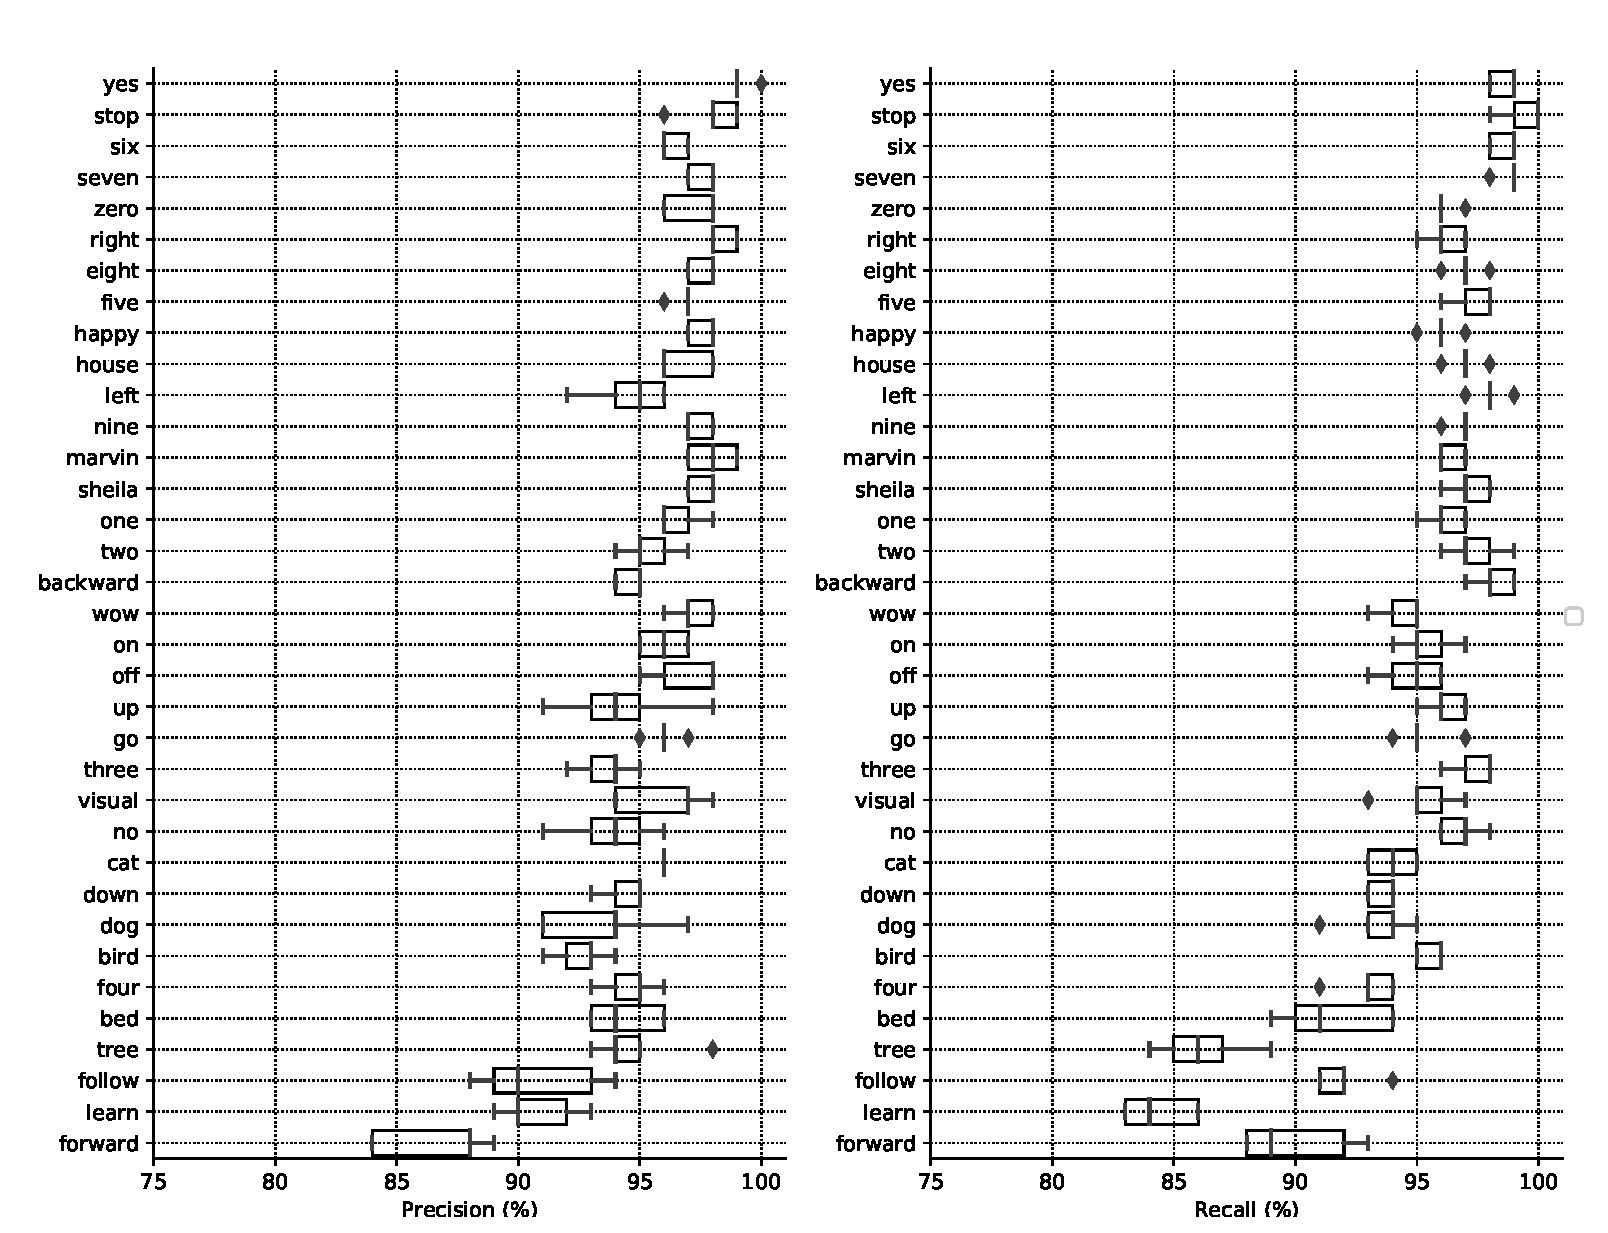
\includegraphics[width=0.8\linewidth]{img/boxplot_35-words-recognition_002.eps}
	\caption{Precision and recall for each of the different classes using the \textit{35-words-recognition} model trained with data version V2. Classes are sorted by descending f1-score.}
	\label{fig:boxplot35002}
\end{figure}
}

\section{Conclusions}
\frame{\frametitle{We suggest Xception-1d as the default architecture for a speech commands classification problem}
\begin{itemize}
    \item We showed how a neural net that succeeded in the computer vision field can be adapted to the speech recognition field and achieve state of the art results
    \item We suggest \textit{Xception-1d} as the \textit{de facto} architecture when facing this kind of task
\end{itemize}
}

\section{Backup}
% --------------------------------------------- NEW SLIDE ------------------------------
\frame{
\centering
\Huge Backup
}

% --------------------------------------------- NEW SLIDE ------------------------------
\subsection{35-words recognition – V1}

\frame{
\tiny
\begin{table}[h!] \centering
    \def\arraystretch{0.85}
	\begin{tabular}{lcccc}
		\toprule
		{} &       precision &          recall &        f1-score & support \\
		\midrule
		happy     &  98.00$\pm$0.89 &  97.80$\pm$0.75 &  98.00$\pm$0.63 &     180 \\
		cat       &  98.20$\pm$0.40 &  97.80$\pm$0.40 &  98.00$\pm$0.00 &     166 \\
		house     &  97.60$\pm$1.36 &  98.60$\pm$0.49 &  97.80$\pm$0.75 &     150 \\
		dog       &  97.80$\pm$0.75 &  98.00$\pm$0.00 &  97.80$\pm$0.40 &     180 \\
		marvin    &  99.00$\pm$0.63 &  96.80$\pm$0.75 &  97.80$\pm$0.40 &     162 \\
		stop      &  97.20$\pm$1.47 &  98.20$\pm$0.40 &  97.60$\pm$1.02 &     249 \\
		yes       &  98.60$\pm$1.02 &  96.40$\pm$0.80 &  97.40$\pm$0.49 &     256 \\
		sheila    &  97.20$\pm$1.33 &  97.00$\pm$0.63 &  97.20$\pm$0.75 &     186 \\
		wow       &  96.80$\pm$1.17 &  97.40$\pm$0.49 &  97.20$\pm$0.40 &     165 \\
		seven     &  95.80$\pm$1.47 &  98.40$\pm$0.80 &  97.20$\pm$0.40 &     239 \\
		four      &  96.40$\pm$0.80 &  97.20$\pm$0.75 &  97.00$\pm$0.63 &     253 \\
		two       &  95.80$\pm$1.33 &  97.60$\pm$0.49 &  96.80$\pm$0.75 &     264 \\
		nine      &  95.40$\pm$1.50 &  98.20$\pm$0.75 &  96.80$\pm$0.40 &     259 \\
		on        &  95.80$\pm$1.60 &  97.00$\pm$0.63 &  96.60$\pm$1.02 &     246 \\
		six       &  95.80$\pm$0.40 &  97.20$\pm$0.40 &  96.40$\pm$0.49 &     244 \\
		bird      &  95.80$\pm$0.98 &  96.40$\pm$0.49 &  96.20$\pm$0.75 &     158 \\
		eight     &  96.80$\pm$1.94 &  95.40$\pm$0.49 &  96.00$\pm$0.89 &     257 \\
		five      &  96.00$\pm$0.63 &  96.00$\pm$0.63 &  96.00$\pm$0.63 &     271 \\
		one       &  98.00$\pm$0.89 &  93.80$\pm$1.33 &  95.80$\pm$0.40 &     248 \\
		down      &  96.00$\pm$0.63 &  95.00$\pm$0.89 &  95.60$\pm$0.80 &     253 \\
		bed       &  95.00$\pm$1.67 &  96.20$\pm$1.47 &  95.40$\pm$1.02 &     176 \\
		left      &  93.00$\pm$1.67 &  97.20$\pm$0.40 &  95.20$\pm$0.75 &     267 \\
		off       &  96.80$\pm$1.47 &  94.00$\pm$1.26 &  95.20$\pm$0.40 &     262 \\
		right     &  97.40$\pm$1.20 &  92.80$\pm$0.40 &  95.20$\pm$0.40 &     259 \\
		zero      &  95.60$\pm$1.36 &  94.40$\pm$1.02 &  95.00$\pm$0.63 &     250 \\
		up        &  94.80$\pm$0.75 &  94.80$\pm$0.98 &  94.80$\pm$0.75 &     272 \\
		no        &  94.60$\pm$1.02 &  93.00$\pm$0.89 &  93.80$\pm$1.17 &     252 \\
		go        &  94.60$\pm$1.62 &  93.40$\pm$0.80 &  93.80$\pm$0.75 &     251 \\
		tree      &  92.40$\pm$1.50 &  90.60$\pm$1.36 &  91.60$\pm$0.49 &     193 \\
		three     &  89.60$\pm$0.49 &  92.80$\pm$0.75 &  91.20$\pm$0.40 &     267 \\
		\midrule avg/total &  96.00$\pm$0.00 &  96.00$\pm$0.00 &  96.00$\pm$0.00 &    6835 \\
		\bottomrule
	\end{tabular}

\end{table}
}

% --------------------------------------------- NEW SLIDE ------------------------------
\subsection{35-words recognition – V2}

\frame{
\tiny
\begin{table}[h!] \centering
    \def\arraystretch{0.85}
	\begin{tabular}{lcccc}
		\toprule
		{} &       precision &          recall &        f1-score & support \\
		\midrule
		yes       &  99.20$\pm$0.40 &  98.60$\pm$0.49 &  99.00$\pm$0.00 &     419 \\
		stop      &  98.00$\pm$1.10 &  99.40$\pm$0.80 &  98.60$\pm$0.49 &     411 \\
		seven     &  97.60$\pm$0.49 &  98.80$\pm$0.40 &  98.40$\pm$0.49 &     406 \\
		six       &  96.40$\pm$0.49 &  98.60$\pm$0.49 &  97.60$\pm$0.49 &     394 \\
		right     &  98.40$\pm$0.49 &  96.20$\pm$0.75 &  97.40$\pm$0.49 &     396 \\
		sheila    &  97.60$\pm$0.49 &  97.20$\pm$0.75 &  97.20$\pm$0.75 &     212 \\
		nine      &  97.40$\pm$0.49 &  96.80$\pm$0.40 &  97.20$\pm$0.40 &     408 \\
		eight     &  97.60$\pm$0.49 &  97.00$\pm$0.63 &  97.20$\pm$0.40 &     408 \\
		marvin    &  98.00$\pm$0.89 &  96.40$\pm$0.49 &  97.20$\pm$0.40 &     195 \\
		five      &  96.80$\pm$0.40 &  97.40$\pm$0.80 &  97.00$\pm$0.00 &     445 \\
		house     &  96.80$\pm$0.98 &  97.00$\pm$0.63 &  96.80$\pm$0.75 &     191 \\
		happy     &  97.60$\pm$0.49 &  96.00$\pm$0.63 &  96.80$\pm$0.40 &     203 \\
		zero      &  97.20$\pm$0.98 &  96.20$\pm$0.40 &  96.60$\pm$0.49 &     418 \\
		left      &  94.60$\pm$1.50 &  98.00$\pm$0.63 &  96.40$\pm$0.80 &     412 \\
		backward  &  94.60$\pm$0.49 &  98.20$\pm$0.75 &  96.40$\pm$0.49 &     165 \\
		one       &  96.60$\pm$0.80 &  96.20$\pm$0.75 &  96.40$\pm$0.49 &     399 \\
		two       &  95.40$\pm$1.02 &  97.40$\pm$1.02 &  96.20$\pm$0.75 &     424 \\
		wow       &  97.20$\pm$0.75 &  94.40$\pm$0.80 &  96.00$\pm$0.89 &     206 \\
		off       &  97.00$\pm$1.26 &  94.80$\pm$1.17 &  95.80$\pm$0.75 &     402 \\
		on        &  96.00$\pm$0.89 &  95.40$\pm$1.02 &  95.80$\pm$0.40 &     396 \\
		visual    &  96.00$\pm$1.67 &  95.20$\pm$1.33 &  95.60$\pm$0.80 &     165 \\
		go        &  96.00$\pm$0.63 &  95.20$\pm$0.98 &  95.40$\pm$0.49 &     402 \\
		no        &  93.80$\pm$1.72 &  96.80$\pm$0.75 &  95.40$\pm$0.49 &     405 \\
		up        &  94.20$\pm$2.32 &  96.20$\pm$0.75 &  95.20$\pm$0.98 &     425 \\
		cat       &  96.00$\pm$0.00 &  94.00$\pm$0.89 &  95.20$\pm$0.75 &     194 \\
		three     &  93.60$\pm$1.02 &  97.40$\pm$0.80 &  95.20$\pm$0.75 &     405 \\
		four      &  94.60$\pm$1.02 &  93.00$\pm$1.10 &  94.00$\pm$0.63 &     400 \\
		bird      &  92.60$\pm$1.02 &  95.60$\pm$0.49 &  94.00$\pm$0.63 &     185 \\
		down      &  94.40$\pm$0.80 &  93.60$\pm$0.49 &  94.00$\pm$0.00 &     406 \\
		dog       &  93.40$\pm$2.24 &  93.40$\pm$1.36 &  93.40$\pm$0.80 &     220 \\
		bed       &  94.40$\pm$1.36 &  91.60$\pm$2.06 &  93.20$\pm$1.17 &     207 \\
		follow    &  90.80$\pm$2.32 &  92.00$\pm$1.10 &  91.60$\pm$1.36 &     172 \\
		tree      &  94.80$\pm$1.72 &  86.20$\pm$1.72 &  90.40$\pm$1.20 &     193 \\
		forward   &  86.60$\pm$2.15 &  90.00$\pm$2.10 &  88.20$\pm$1.72 &     155 \\
		learn     &  90.80$\pm$1.47 &  84.40$\pm$1.36 &  87.60$\pm$1.02 &     161 \\
		\midrule avg/total &  96.00$\pm$0.00 &  96.00$\pm$0.00 &  96.00$\pm$0.00 &   11005 \\
		\bottomrule
	\end{tabular}

\end{table}
}

% --------------------------------------------- NEW SLIDE ------------------------------
\subsection{20-commands recognition – V1}
\frame{
\tiny
\begin{table} \centering
	\caption{Detailed results for task \textit{20-commands-recognition} and data version V1, sorted by decreasing f1-score order. The columns ``precision'', ``recall'' and ``f1-score'' have been represented as the mean $\pm$ the standard deviation in percentage scale. }
	\begin{tabular}{lcccc}
		\toprule
		{} &       precision &          recall &        f1-score & support \\
		\midrule
		nine      &  97.80$\pm$1.17 &  97.60$\pm$1.02 &  97.80$\pm$0.40 &     259 \\
		stop      &  97.00$\pm$1.79 &  98.00$\pm$0.63 &  97.60$\pm$1.02 &     249 \\
		yes       &  98.60$\pm$0.80 &  96.40$\pm$0.49 &  97.60$\pm$0.49 &     256 \\
		seven     &  96.40$\pm$0.49 &  98.20$\pm$0.75 &  97.40$\pm$0.49 &     239 \\
		six       &  97.20$\pm$0.75 &  97.40$\pm$0.49 &  97.20$\pm$0.40 &     244 \\
		unknown   &  96.60$\pm$0.49 &  97.00$\pm$0.00 &  97.00$\pm$0.00 &    1716 \\
		on        &  96.40$\pm$1.20 &  97.20$\pm$0.40 &  96.80$\pm$0.40 &     246 \\
		five      &  96.80$\pm$1.17 &  95.60$\pm$0.80 &  96.20$\pm$0.75 &     271 \\
		one       &  98.00$\pm$0.63 &  94.20$\pm$0.40 &  96.20$\pm$0.40 &     248 \\
		zero      &  96.60$\pm$1.50 &  94.60$\pm$1.02 &  95.80$\pm$0.98 &     250 \\
		four      &  94.00$\pm$1.10 &  97.60$\pm$0.49 &  95.80$\pm$0.75 &     253 \\
		two       &  94.80$\pm$1.60 &  96.40$\pm$0.80 &  95.60$\pm$1.02 &     264 \\
		left      &  93.60$\pm$1.02 &  97.20$\pm$0.75 &  95.40$\pm$0.80 &     267 \\
		eight     &  95.60$\pm$0.49 &  95.40$\pm$0.80 &  95.40$\pm$0.49 &     257 \\
		right     &  96.60$\pm$1.02 &  93.80$\pm$1.17 &  95.20$\pm$0.98 &     259 \\
		off       &  97.20$\pm$1.17 &  93.60$\pm$1.02 &  95.20$\pm$0.75 &     262 \\
		up        &  95.80$\pm$0.40 &  94.40$\pm$1.50 &  95.00$\pm$0.63 &     272 \\
		down      &  95.80$\pm$0.75 &  93.40$\pm$0.80 &  94.60$\pm$0.49 &     253 \\
		no        &  93.20$\pm$1.33 &  94.80$\pm$0.75 &  94.00$\pm$0.63 &     252 \\
		go        &  94.00$\pm$1.55 &  91.40$\pm$1.62 &  92.60$\pm$0.49 &     251 \\
		three     &  91.00$\pm$0.89 &  92.00$\pm$1.55 &  91.40$\pm$1.02 &     267 \\
		\midrule avg/total &  96.00$\pm$0.00 &  96.00$\pm$0.00 &  96.00$\pm$0.00 &    6835 \\
		\bottomrule
	\end{tabular}

\end{table}

}

% --------------------------------------------- NEW SLIDE ------------------------------
\subsection{20-commands recognition – V2}
\frame{
\tiny

\begin{table} \centering
	\caption{Detailed results for task \textit{20-commands-recognition} and data version V2, sorted by decreasing f1-score order. The columns ``precision'', ``recall'' and ``f1-score'' have been represented as the mean $\pm$ the standard deviation in percentage scale. }
	\begin{tabular}{lcccc}
		\toprule
		{} &       precision &          recall &        f1-score & support \\
		\midrule
		seven     &  98.80$\pm$0.40 &  98.60$\pm$0.49 &  98.80$\pm$0.40 &     406 \\
		yes       &  98.80$\pm$0.40 &  98.60$\pm$0.49 &  98.60$\pm$0.49 &     419 \\
		stop      &  98.80$\pm$0.40 &  99.00$\pm$0.63 &  98.60$\pm$0.49 &     411 \\
		six       &  97.60$\pm$1.02 &  98.20$\pm$0.75 &  97.60$\pm$0.49 &     394 \\
		eight     &  98.00$\pm$0.63 &  96.40$\pm$0.49 &  97.00$\pm$0.00 &     408 \\
		zero      &  97.80$\pm$0.75 &  96.40$\pm$0.49 &  96.80$\pm$0.40 &     418 \\
		nine      &  98.00$\pm$0.63 &  95.40$\pm$0.49 &  96.60$\pm$0.49 &     408 \\
		right     &  97.40$\pm$1.36 &  96.00$\pm$0.89 &  96.60$\pm$0.49 &     396 \\
		two       &  95.80$\pm$0.75 &  96.80$\pm$0.75 &  96.40$\pm$0.49 &     424 \\
		five      &  96.60$\pm$1.02 &  95.40$\pm$1.20 &  96.00$\pm$0.63 &     445 \\
		one       &  97.40$\pm$0.49 &  95.00$\pm$0.00 &  96.00$\pm$0.00 &     399 \\
		left      &  94.40$\pm$0.80 &  97.60$\pm$0.49 &  96.00$\pm$0.00 &     412 \\
		off       &  97.20$\pm$0.75 &  94.60$\pm$1.20 &  95.80$\pm$0.75 &     402 \\
		no        &  95.20$\pm$1.47 &  96.40$\pm$0.49 &  95.80$\pm$0.75 &     405 \\
		on        &  95.60$\pm$1.62 &  95.20$\pm$0.75 &  95.40$\pm$0.49 &     396 \\
		up        &  95.40$\pm$0.49 &  95.20$\pm$0.40 &  95.40$\pm$0.49 &     425 \\
		three     &  94.40$\pm$1.02 &  96.20$\pm$1.17 &  95.00$\pm$0.00 &     405 \\
		unknown   &  94.40$\pm$0.49 &  96.00$\pm$0.63 &  95.00$\pm$0.00 &    2824 \\
		go        &  95.00$\pm$1.41 &  94.80$\pm$0.75 &  94.80$\pm$0.40 &     402 \\
		down      &  94.80$\pm$0.40 &  93.40$\pm$0.49 &  94.20$\pm$0.40 &     406 \\
		four      &  95.20$\pm$0.98 &  92.00$\pm$1.67 &  93.60$\pm$0.49 &     400 \\
		\midrule avg/total &  96.00$\pm$0.00 &  96.00$\pm$0.00 &  96.00$\pm$0.00 &   11005 \\
		\bottomrule
	\end{tabular}

\end{table}
}

% --------------------------------------------- NEW SLIDE ------------------------------
\subsection{10-commands recognition – V1}
\frame{
\tiny
\begin{table} \centering \scriptsize
	\caption{Detailed results for task \textit{10-commands-recognition} and data version V1, sorted by decreasing f1-score order. The columns ``precision'', ``recall'' and ``f1-score'' have been represented as the mean $\pm$ the standard deviation in percentage scale. }
	\begin{tabular}{lcccc}
		\toprule
		{} &       precision &          recall &        f1-score & support \\
		\midrule
		unknown   &  97.60$\pm$0.49 &  99.00$\pm$0.00 &  98.20$\pm$0.40 &    4268 \\
		stop      &  98.20$\pm$1.17 &  97.60$\pm$0.80 &  97.80$\pm$0.40 &     249 \\
		yes       &  98.60$\pm$1.50 &  95.60$\pm$0.80 &  97.00$\pm$0.89 &     256 \\
		on        &  97.60$\pm$1.02 &  95.80$\pm$0.40 &  96.80$\pm$0.40 &     246 \\
		left      &  95.60$\pm$1.02 &  95.60$\pm$0.80 &  95.60$\pm$0.49 &     267 \\
		right     &  96.60$\pm$1.50 &  92.80$\pm$0.75 &  94.40$\pm$0.80 &     259 \\
		up        &  95.60$\pm$1.36 &  93.00$\pm$0.89 &  94.40$\pm$0.80 &     272 \\
		off       &  96.40$\pm$1.50 &  92.40$\pm$1.50 &  94.40$\pm$0.49 &     262 \\
		down      &  95.40$\pm$0.49 &  92.80$\pm$0.75 &  94.20$\pm$0.40 &     253 \\
		no        &  94.80$\pm$0.75 &  91.80$\pm$0.40 &  93.20$\pm$0.40 &     252 \\
		go        &  93.60$\pm$2.24 &  92.40$\pm$1.62 &  92.80$\pm$1.33 &     251 \\
		\midrule avg/total &  97.00$\pm$0.00 &  97.00$\pm$0.00 &  97.00$\pm$0.00 &    6835 \\
		\bottomrule
	\end{tabular}

\end{table}
}

% --------------------------------------------- NEW SLIDE ------------------------------
\subsection{20-commands recognition – V2}
\frame{
\tiny
\begin{table} \centering \scriptsize
	\caption{Detailed results for task \textit{10-commands-recognition} and data version V2, sorted by decreasing f1-score order. The columns ``precision'', ``recall'' and ``f1-score'' have been represented as the mean $\pm$ the standard deviation in percentage scale. }
	\begin{tabular}{lcccc}
		\toprule
		{} &       precision &          recall &        f1-score & support \\
		\midrule
		unknown   &  98.20$\pm$0.40 &  99.00$\pm$0.00 &  99.00$\pm$0.00 &    6931 \\
		yes       &  99.00$\pm$0.63 &  98.40$\pm$0.49 &  98.80$\pm$0.40 &     419 \\
		stop      &  98.40$\pm$0.49 &  98.60$\pm$0.49 &  98.40$\pm$0.49 &     411 \\
		right     &  97.80$\pm$0.75 &  95.60$\pm$1.02 &  96.80$\pm$0.75 &     396 \\
		left      &  94.40$\pm$1.02 &  97.40$\pm$0.49 &  95.80$\pm$0.40 &     412 \\
		go        &  95.40$\pm$1.02 &  94.80$\pm$0.75 &  95.00$\pm$0.63 &     402 \\
		up        &  96.20$\pm$0.75 &  93.60$\pm$0.49 &  95.00$\pm$0.00 &     425 \\
		no        &  93.80$\pm$1.33 &  95.20$\pm$1.33 &  94.80$\pm$0.75 &     405 \\
		off       &  95.40$\pm$0.80 &  93.80$\pm$0.40 &  94.60$\pm$0.49 &     402 \\
		on        &  95.60$\pm$1.02 &  93.80$\pm$0.75 &  94.40$\pm$0.49 &     396 \\
		down      &  94.80$\pm$0.98 &  93.00$\pm$0.89 &  94.00$\pm$0.63 &     406 \\
		\midrule avg/total &  97.60$\pm$0.49 &  97.60$\pm$0.49 &  97.60$\pm$0.49 &   11005 \\
		\bottomrule
	\end{tabular}

\end{table}
}

% --------------------------------------------- NEW SLIDE ------------------------------
\subsection{left-right recognition – V1 and V2}
\frame{
\tiny

\begin{table} \centering \scriptsize
	\caption{Detailed results for task \textit{left-right} and data version V1, sorted by decreasing f1-score order. The columns ``precision'', ``recall'' and ``f1-score'' have been represented as the mean $\pm$ the standard deviation in percentage scale. }
	\begin{tabular}{lcccc}
		\toprule
		{} &       precision &           recall &        f1-score & support \\
		\midrule
		unknown   &  99.00$\pm$0.00 &  100.00$\pm$0.00 &  99.20$\pm$0.40 &    6309 \\
		left      &  95.40$\pm$1.96 &   92.00$\pm$0.89 &  93.60$\pm$0.80 &     267 \\
		right     &  96.20$\pm$1.94 &   87.60$\pm$1.85 &  91.80$\pm$0.75 &     259 \\
		\midrule avg/total &  99.00$\pm$0.00 &   99.00$\pm$0.00 &  99.00$\pm$0.00 &    6835 \\
		\bottomrule
	\end{tabular}

\end{table}

\begin{table} \centering \scriptsize
	\caption{Detailed results for task \textit{left-right} and data version V2, sorted by decreasing f1-score order. The columns ``precision'', ``recall'' and ``f1-score'' have been represented as the mean $\pm$ the standard deviation in percentage scale. }
	\begin{tabular}{lcccc}
		\toprule
		{} &       precision &           recall &         f1-score & support \\
		\midrule
		unknown   &  99.40$\pm$0.49 &  100.00$\pm$0.00 &  100.00$\pm$0.00 &   10197 \\
		left      &  95.80$\pm$0.98 &   94.00$\pm$0.89 &   95.00$\pm$0.63 &     412 \\
		right     &  98.20$\pm$1.47 &   90.60$\pm$2.65 &   94.00$\pm$1.10 &     396 \\
		\midrule avg/total &  99.00$\pm$0.00 &   99.00$\pm$0.00 &   99.00$\pm$0.00 &   11005 \\
		\bottomrule
	\end{tabular}

\end{table}
}

\end{document}
